\documentclass[letterpaper,11pt]{article}

% Packages
\usepackage[utf8]{inputenc}
\usepackage[T1]{fontenc}
\usepackage[margin=0.75in]{geometry}
\usepackage{hyperref}
\usepackage{enumitem}
\usepackage{titlesec}
\usepackage{xcolor}
\usepackage{fontawesome5}
\usepackage{tikz}
\usepackage{graphicx}
\usepackage{multicol}

% Color definitions
\definecolor{accent}{RGB}{230, 126, 34}
\definecolor{dark}{RGB}{44, 62, 80}
\definecolor{light}{RGB}{149, 165, 166}
\definecolor{white}{RGB}{255, 255, 255}

% Hyperlink setup
\hypersetup{
    colorlinks=true,
    linkcolor=accent,
    urlcolor=accent,
    citecolor=accent
}

% Custom commands
\newcommand{\sectiontitle}[1]{
    \vspace{0.5em}
    \begin{tikzpicture}
        \node[fill=accent, text=white, font=\Large\bfseries, inner sep=8pt, minimum width=\textwidth-16pt] {#1};
    \end{tikzpicture}
    \vspace{0.3em}
}

\newcommand{\jobentry}[4]{
    \textcolor{dark}{\textbf{#1}} \hfill \textcolor{accent}{\textbf{#2}} \\
    \textcolor{light}{\textit{#3}} \hfill \textcolor{light}{#4}
}

\newcommand{\highlight}[1]{\textcolor{accent}{\textbf{#1}}}

% Remove page numbers
\pagestyle{empty}

% Adjust spacing
\setlength{\parindent}{0pt}
\setlength{\parskip}{0.4em}

\begin{document}

% Header with creative design
\begin{center}
    
\begin{tikzpicture}
        \node[fill=dark, text=white, font=\Huge\bfseries, inner sep=12pt, minimum width=\textwidth-24pt] {{{ profile.name | default("JOHN DOE") }}};
    \end{tikzpicture}
    
    \vspace{0.3em}
    
    \textcolor{dark}{
        \faEnvelope \, {{ profile.email | default("john.doe@example.com") }} \quad
        \faPhone \, {{ profile.phone | default("(555) 123-4567") }} \quad
        \faMapMarker \, {{ profile.location | default("City, State") }}
    }
    
    
    \vspace{0.2em}
    \textcolor{accent}{\faLinkedin \, {{ profile.linkedin_url }}}
    
\end{center}

% Professional Summary

\sectiontitle{PROFESSIONAL SUMMARY}
\textcolor{dark}{{{ profile.summary | default("Creative and results-driven professional with a passion for innovation and excellence in technology solutions.") }}}


% Experience

\sectiontitle{PROFESSIONAL EXPERIENCE}


\jobentry{ {{ experience.title }} }{ {{ experience.duration }} }{ {{ experience.company }} }{ {{ experience.location | default("") }} }

\begin{itemize}[leftmargin=1em, itemsep=0.3em]
    
    \item \textcolor{dark}{ {{ responsibility }} }
    
\end{itemize}

\vspace{0.4em}


% Default experience if no data

\jobentry{Creative Developer}{2020 - Present}{Innovative Tech Solutions}{San Francisco, CA}

\begin{itemize}[leftmargin=1em, itemsep=0.3em]
    \item \textcolor{dark}{Designed and developed cutting-edge web applications with focus on user experience}
    \item \textcolor{dark}{Led creative initiatives resulting in 40\% increase in user engagement}
    \item \textcolor{dark}{Collaborated with design teams to implement innovative interface solutions}
\end{itemize}

\vspace{0.4em}




% Education

\sectiontitle{EDUCATION}


\jobentry{ {{ education.degree }} }{ {{ education.year }} }{ {{ education.institution }} }{ {{ education.location | default("") }} }


\textcolor{light}{GPA: {{ education.gpa }}}


\vspace{0.4em}


% Default education if no data

\jobentry{Bachelor of Arts in Digital Media}{2020}{Creative Arts University}{Los Angeles, CA}

\textcolor{light}{Magna Cum Laude, GPA: 3.8/4.0}

\vspace{0.4em}




% Skills with creative layout

\sectiontitle{CORE COMPETENCIES}

\begin{multicols}{2}
\begin{itemize}[leftmargin=1em, itemsep=0.2em]
    
    \item \highlight{ {{ skill }} }
    
    
    
    \item \highlight{Creative Design}
    \item \highlight{Web Development}
    \item \highlight{User Experience}
    \item \highlight{Project Management}
    \item \highlight{Brand Strategy}
    \item \highlight{Digital Marketing}
    \item \highlight{Content Creation}
    \item \highlight{Team Leadership}
    
\end{itemize}
\end{multicols}



% Projects

\sectiontitle{FEATURED PROJECTS}


\begin{tikzpicture}
    \node[fill=light!20, inner sep=8pt, minimum width=\textwidth-16pt] {
        \begin{minipage}{\textwidth-32pt}
            \textcolor{dark}{\textbf{ {{ project.name }} }} \hfill \textcolor{accent}{ {{ project.duration }} }
            
            \textcolor{dark}{ {{ project.description }} }
            
            \begin{itemize}[leftmargin=1em, itemsep=0.2em, topsep=0.3em]
                
                \item \textcolor{dark}{ {{ detail }} }
                
            \end{itemize}
        \end{minipage}
    };
\end{tikzpicture}

\vspace{0.3em}


% Default project if no data

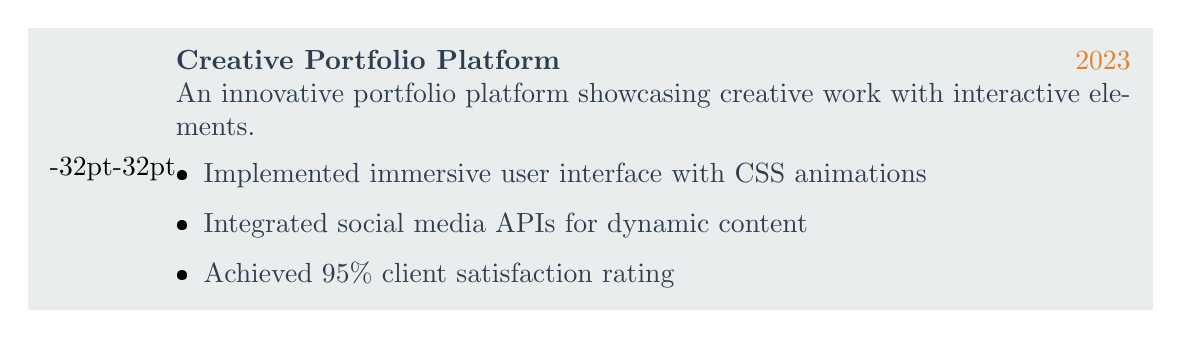
\begin{tikzpicture}
    \node[fill=light!20, inner sep=8pt, minimum width=\textwidth-16pt] {
        \begin{minipage}{\textwidth-32pt}
            \textcolor{dark}{\textbf{Creative Portfolio Platform}} \hfill \textcolor{accent}{2023}
            
            \textcolor{dark}{An innovative portfolio platform showcasing creative work with interactive elements.}
            
            \begin{itemize}[leftmargin=1em, itemsep=0.2em, topsep=0.3em]
                \item \textcolor{dark}{Implemented immersive user interface with CSS animations}
                \item \textcolor{dark}{Integrated social media APIs for dynamic content}
                \item \textcolor{dark}{Achieved 95\% client satisfaction rating}
            \end{itemize}
        \end{minipage}
    };
\end{tikzpicture}

\vspace{0.3em}




% Certifications

\sectiontitle{CERTIFICATIONS \& ACHIEVEMENTS}


\textcolor{dark}{\textbf{ {{ cert.name }} }} \hfill \textcolor{accent}{ {{ cert.issuer }} , {{ cert.date }} }


\textcolor{light}{Credential ID: {{ cert.credential_id }}}


\vspace{0.3em}


% Default certification if no data

\textcolor{dark}{\textbf{Adobe Certified Expert}} \hfill \textcolor{accent}{Adobe, 2023}

\textcolor{light}{Credential ID: ACE-456789}

\vspace{0.3em}




\end{document}
